\documentclass[12pt]{article}
\usepackage{pbox}
\usepackage{graphicx}
\usepackage{url}
\usepackage{booktabs}
\usepackage[table,xcdraw]{xcolor}
 \usepackage[normalem]{ulem}
 \usepackage{marginnote}
 \usepackage{geometry}
 \useunder{uline}{\ul}{}
\title{Amended timescale for PhD}
\author{
        Lewis Sharpe}
\date{\today}

\begin{document}
\maketitle
\section{Project Timeline:}
Due to numerous complications and delays in my study, a revised timeline until PhD completion has been compiled. The revised submission date for the PhD Thesis has been made for August 2021. You can see a progression diagram and a table schedule of new projected timeline below.
\subsection{Description of Project Phases:}
\colorbox{blue!30}{\textbf{Phase 1: Design of Minimax algorithm variants:}} \\
The first phase would design an Minimax algorithm with sequential and parallel variants, measure and compare the speed up achieved between them, then tuning algorithms to see if this speed up can be improved.  \\
\colorbox{green!30}{\textbf{Phase 2: Fitting Minimax into a larger game scenario:}} \\
The second phase would look to embed the above algorithm in larger logic game, and perform an experiment to observe how it performs with complexer decisions to make. \\
\colorbox{orange!30}{\textbf{Phase 3: Determining degree of Correlation between two factors:}} \\
The third phase will look to conduct experiment that would assess degree of correlation between 1) the increased performance of an AI search gained through parallelism (in Phase 2), and 2) a player's view of increased engagement in gameplay (assessed in Phase 3).  \\
\colorbox{gray!30}{\textbf{Phase 4: Write-up:}} \\
The final stage will be to write up and sum the whole research, and aim to cogent an argument to prove or disapprove a correlation between 1) the increased performance of an AI search gained through parallelism, and 2) a player's view of increased engagement in gameplay.
\subsection{Full revised project timeline represented as a progression diagram:}
\begin{flushleft}
   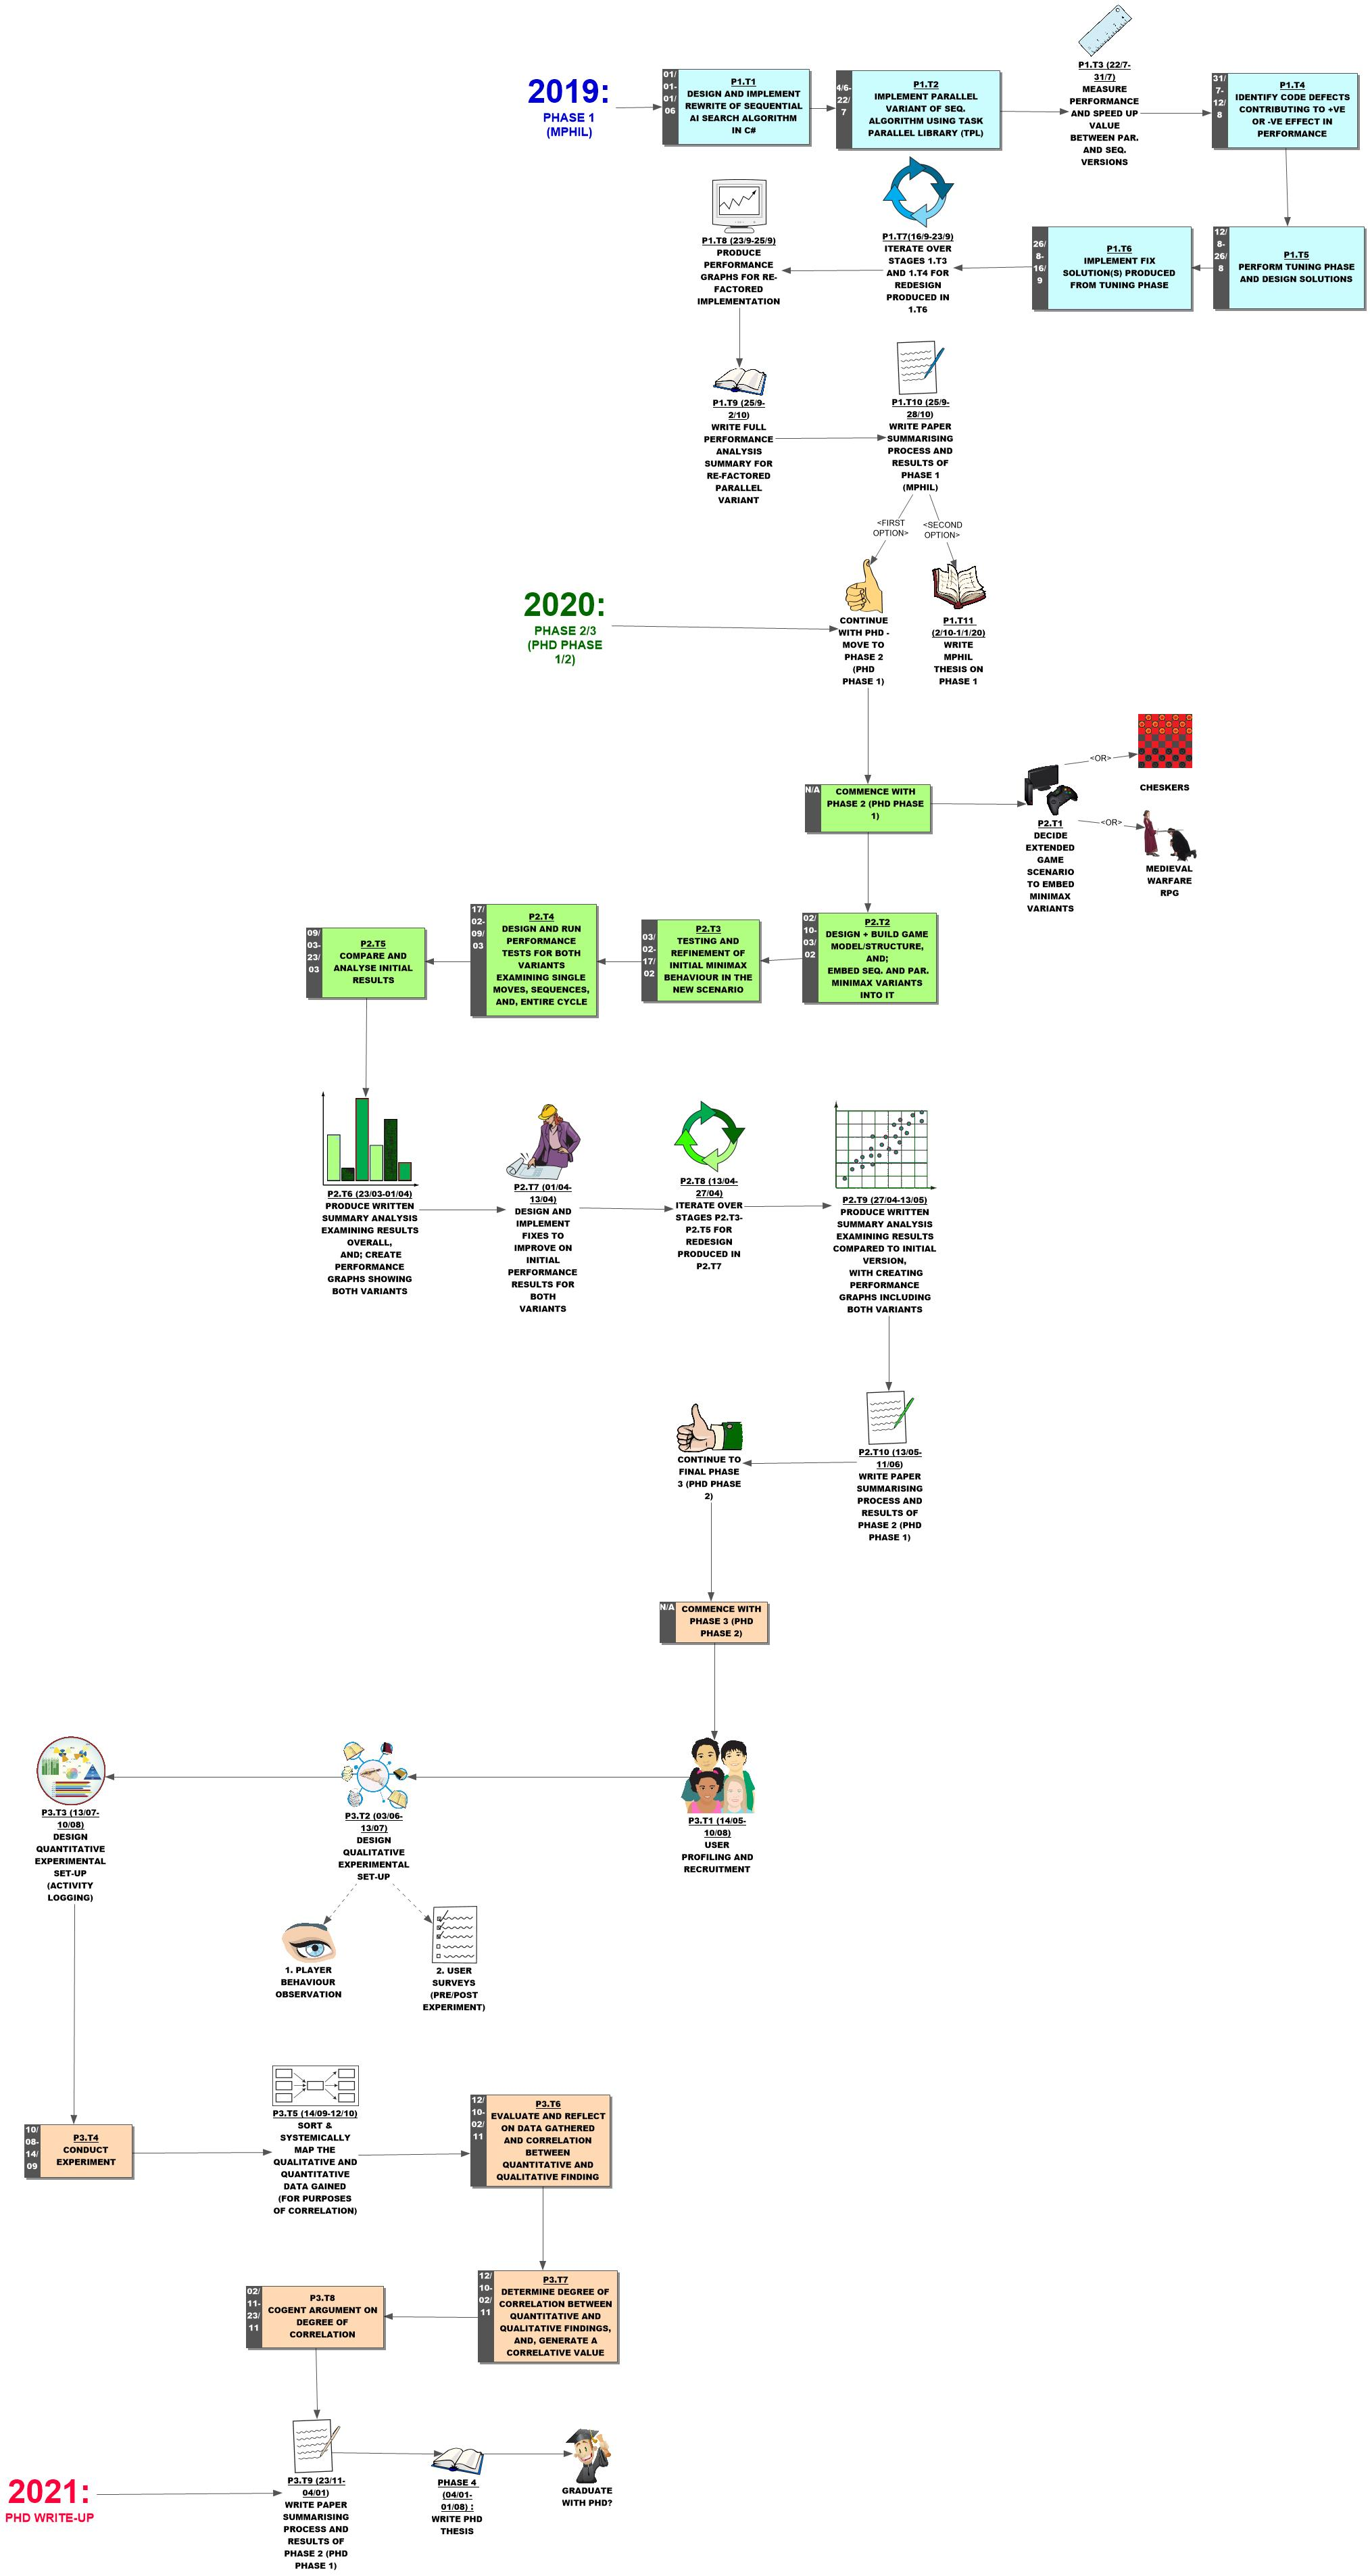
\includegraphics[width=0.8\linewidth]{phd_plan_july19.jpg}
\end{flushleft}
\subsection{Full revised project timeline represented in table format:}
A full table of contents embodying the projected work schedule is presented below.
\begin{center}
     \begin{tabular}{ | l | l | l | l | l | p{10cm} |}
    \hline
       \textbf{P} & \textbf{NO.} & \textbf{TASK} & \textbf{START} & \textbf{END}
    \\ \hline
  \colorbox{blue!30}{1} & T1 & Design and build rewrite of seq. MiniMax &    01-01-19 &
     01-06-19 \\ \hline
      \colorbox{blue!30}{1} & T2 & Implement TPL parallel variant of seq. Minimax & 04-06-19 & 22-07-19 \\ \hline
      \colorbox{blue!30}{1} & T3 & Measure performance between par. and seq. variants & 22-07-19 & 31-07-19 \\ \hline
       \colorbox{blue!30}{1} & T4 & Identify defects giving +VE or -VE effect on performance & 31-07-19 & 12-08-19 \\ \hline
          \colorbox{blue!30}{1} & T5 & Perform tuning phase and design solutions & 12-08-19 & 26-08-19 \\ \hline
          \colorbox{blue!30}{1} & T6 & Implement fix solution(s) gathered in tuning phase & 26-08-19 & 16-09-19 \\ \hline
           \colorbox{blue!30}{1} & T7 & Iterate over tasks T3 and T4 for T6 re-factored algorithm & 16-09-19 & 23-09-19 \\ \hline
       \colorbox{blue!30}{1} & T8 & Produce performance graphs for re-factored implementation & 23-09-19 & 25-09-19 \\ \hline
     \colorbox{blue!30}{1} & T9 & Write performance analysis for re-factored parallel variant & 25-09-19 & 02-10-19 \\ \hline
      \colorbox{blue!30}{1} & T10 & Write paper summarising process and results of phase & 25-09-19 & 28-10-19
  \\ \hline
     \colorbox{green!30}{2} & T1 & Decide extended game scenario to embed Minimax variants in & 23-09-19 & 07-10-19
       \\ \hline
       \colorbox{green!30}{2} & T2 & Design/build game-model + embed Minimax variants within & 02-10-19 & 03-02-20
       \\ \hline
              \colorbox{green!30}{2} & T3 & Testing and refinement of Minimax in new scenario & 03-02-20 & 17-02-20
       \\ \hline
             \colorbox{green!30}{2} & T4 & Performance testing for both variants & 17-02-20 & 09-03-20
       \\ \hline
         \colorbox{green!30}{2} & T5 & Compare and analyse initial results & 09-03-20 & 23-03-20
           \\ \hline
         \colorbox{green!30}{2} & T6 & Write performance analysis summary with speed-up graphs & 23-03-20 & 01-04-20
       \\ \hline
       \colorbox{green!30}{2} & T7 & Design and build fixes to improve on initial performance results & 01-04-20 & 13-04-20
       \\ \hline
        \colorbox{green!30}{2} & T8 & Iterate over T3-T6 for T7 re-factored version & 13-04-20 & 27-04-20
           \\ \hline
            \colorbox{green!30}{2} & T9 & Write re-factored performance analysis with speed-up graphs & 27-04-20 & 13-05-20
       \\ \hline
        \colorbox{green!30}{2} & T10 & Write paper summarising process and results of phase & 13-05-20 & 11-06-20
       \\ \hline
    \colorbox{orange!30}{3} & T1 & User Profiling and Recruitment & 14-05-20 & 10-08-20
       \\ \hline
       \colorbox{orange!30}{3} & T2 & Design Qualitative experiment set-up & 03-06-20 & 13-07-20
       \\ \hline
         \colorbox{orange!30}{3} & T3 & Design Quantitative experiment set-up (activity logging) & 13-07-20 & 10-08-20
       \\ \hline
         \colorbox{orange!30}{3} & T4 & Conduct experiment & 10-08-20 & 14-09-20
       \\ \hline
         \colorbox{orange!30}{3} & T5 & Systemically map the qualitative and quantitative data gained  & 14-09-20 & 12-10-20
       \\ \hline
        \colorbox{orange!30}{3} & T6 & Evaluate data + correlations between quant. and qual. findings  & 12-10-20 & 02-11-20
       \\ \hline
       \colorbox{orange!30}{3} & T7 & Generate correlative value between quant. and qual. findings  & 12-10-20 & 02-11-20
       \\ \hline
       \colorbox{orange!30}{3} & T8 & Cogent argument on degree of correlation  & 02-11-20 & 23-11-20
       \\ \hline
       \colorbox{orange!30}{3} & T9 & Write paper summarising process and results of phase &  23-11-20 & 04-01-21
       \\ \hline
   \colorbox{gray!30}{4} & T10 & Write PhD Thesis  & 04-01-21 & 01-08-21
    \\ \hline
    \end{tabular}
    Table 1: Projected PhD work schedule for remaining work packets
\end{center}
The following citation referring to the template used to create this document. \cite{Gil:02}.
\bibliographystyle{abbrv}
\bibliography{simple}

\end{document}

This is never printed
